\documentclass[11pt, oneside]{article}   	% use "amsart" instead of "article" for AMSLaTeX format
\usepackage[left= 1in, right= 1in, top=1in, bottom=1in]{geometry}                		% See geometry.pdf to learn the layout options. There are lots.
\geometry{letterpaper}                   		% ... or a4paper or a5paper or ... 
%\geometry{landscape}                		% Activate for rotated page geometry
\usepackage[parfill]{parskip}    		% Activate to begin paragraphs with an empty line rather than an indent
\usepackage{graphicx}				% Use pdf, png, jpg, or eps§ with pdflatex; use eps in DVI mode
								% TeX will automatically convert eps --> pdf in pdflatex		
\usepackage{amssymb}
\usepackage{float}
\usepackage{subcaption}


%SetFonts

%SetFonts


\title{Assignment 1: Local Search}
\author{Jack LoCasto and Andrew Leonard}
\date{September 26, 2017}							% Activate to display a given date or no date

\begin{document}
\maketitle

\section{Task 1}
We used java to produce our GUI for Local Search. The Task 1-2 text field asks the user to input the dimensions of the grid the user wishes to generate. If the user inputs a number that isn't 5, 7, 9, or 11, Local Search pops up a window telling the user their input was incorrect. The generate button completes this process and outputs a grid to the middle of the screen and tells the user if there is a path to the goal in the grid.

\section{Task 2}
Task 2 is completed by pressing the solve button. This outputs a new grid which displays the minimum distance by depth from the start cell to each cell including the goal which defines the evaluation of the grid. The evaluation is then output underneath the grid for the user to see.

We also included another text field that allows the user to input a file containing the dimensions and data for the grid which Local Search generates and solves as well.\\
\\
5x5 Grid Examples:\\
\\
Ex1.txt\\
$
\left[
	\begin{array}{ccccc}
		1&4&2&2&4\\
		3&1&2&3&2\\
		2&1&1&1&3\\
		2&1&3&3&2\\
		4&2&4&4&0\\
	\end{array}
\right]
$
$
\left[
	\begin{array}{ccccc}
		0&1&6&4&7\\
		1&4&5&2&6\\
		4&3&4&5&6\\
		5&4&5&6&7\\
		2&2&X&3&3\\
	\end{array}
\right]
$\\
There is a Path  |  Value Function: 3\\
\\
Ex2.txt\\
$
\left[
	\begin{array}{ccccc}
		4&3&1&4&1\\
		1&1&2&1&1\\
		2&3&1&2&3\\
		4&1&3&3&3\\
		2&2&1&3&0\\
	\end{array}
\right]
$
$
\left[
	\begin{array}{ccccc}
		0&5&4&2&1\\
		5&6&4&3&2\\
		2&4&3&4&3\\
		7&6&3&X&8\\
		1&3&2&3&X\\
	\end{array}
\right]
$\\
There is no Path  |  Value Function: -2\\
\\

7x7 Grid Examples:\\
\\
Ex3.txt\\
$
\left[
	\begin{array}{ccccccc}
		2&6&5&6&2&1&6\\
		5&2&5&2&4&2&2\\
		5&6&1&2&3&4&2\\
		1&2&3&1&2&1&3\\
		4&4&3&4&2&4&4\\
		3&5&5&4&3&2&6\\
		1&2&1&3&4&4&0\\
	\end{array}
\right]
$
$
\left[
	\begin{array}{ccccccc}
		0&6&1&8&8&7&8\\
		9&10&X&9&8&8&X\\
		1&3&X&7&9&2&X\\
		X&11&7&6&7&8&8\\
		X&5&X&7&X&6&X\\
		7&9&2&8&8&X&10\\
		6&4&8&5&X&3&6\\
	\end{array}
\right]
$\\
There is a Path  |  Value Function: 6\\
\\
Ex4.txt\\
$
\left[
	\begin{array}{ccccccc}
		6&3&6&6&1&5&1\\
		1&1&1&5&1&4&2\\
		2&1&4&3&1&2&6\\
		4&5&1&2&4&2&5\\
		5&1&2&4&2&1&4\\
		1&2&4&2&4&4&1\\
		5&2&3&1&1&6&0\\
	\end{array}
\right]
$
$
\left[
	\begin{array}{ccccccc}
		0&4&5&5&4&2&1\\
		2&3&4&4&3&4&2\\
		3&4&4&5&4&5&5\\
		6&4&6&6&5&6&3\\
		4&X&7&X&6&5&6\\
		8&4&X&5&7&3&X\\
		1&X&5&5&6&2&X\\
	\end{array}
\right]
$\\
There is no Path  |  Value Function: -6\\
\\
9x9 Grid Examples:\\
\\
Ex5.txt\\
$
\left[
	\begin{array}{ccccccccc}
		2&6&5&3&7&1&7&1&7\\
		3&3&1&3&6&5&6&2&8\\
		8&6&2&3&1&1&3&6&7\\
		8&4&2&4&1&2&1&1&5\\
		1&2&6&1&3&4&4&3&1\\
		2&4&2&4&3&4&4&3&1\\
		7&6&3&5&5&2&3&6&3\\
		6&7&5&7&6&5&7&2&3\\
		6&3&8&1&6&8&5&6&0\\
	\end{array}
\right]
$
$
\left[
	\begin{array}{ccccccccc}
		0&4&1&7&8&7&3&2&3\\
		5&5&4&5&5&4&6&3&X\\
		1&3&4&5&4&5&6&4&2\\
		4&X&3&5&4&5&5&4&5\\
		6&6&5&6&5&6&6&5&5\\
		3&4&2&6&3&5&7&4&6\\
		X&5&X&6&X&5&X&6&7\\
		4&X&3&6&6&5&4&4&4\\
		X&4&X&X&4&6&7&5&6\\
	\end{array}
\right]
$
\\
There is a Path  |  Value Function: 6\\
\\
Ex6.txt\\
$
\left[
	\begin{array}{ccccccccc}
		7&8&1&8&5&5&5&4&4\\
		1&2&5&7&3&4&5&3&7\\
		3&4&1&6&6&3&1&6&4\\
		8&6&5&4&5&1&5&3&4\\
		2&2&1&4&4&5&6&4&1\\
		3&2&1&5&3&5&2&5&6\\
		3&6&5&1&3&5&2&5&6\\
		7&5&7&2&3&5&3&2&8\\
		3&2&5&7&1&2&8&7&0\\
	\end{array}
\right]
$
$
\left[
	\begin{array}{ccccccccc}
		0&8&X&2&7&6&X&1&7\\
		X&6&6&4&5&10&X&4&X\\
		6&6&5&6&6&4&X&X&5\\
		9&6&6&X&8&X&X&7&8\\
		7&6&5&3&6&X&8&2&7\\
		5&5&4&5&8&5&X&3&6\\
		8&7&5&9&10&9&X&6&6\\
		1&6&X&8&8&3&7&2&9\\
		4&9&7&3&7&8&X&3&X\\
	\end{array}
\right]
$
\\
There is no Path  |  Value Function: -16\\
\\
11x11 Grid Examples:\\
\\
Ex7.txt\\
$
\left[
	\begin{array}{ccccccccccc}
		7&4&10&2&10&6&2&10&2&6&7\\
		2&5&8&8&1&1&1&8&5&6&6\\
		1&3&3&3&6&3&7&2&5&3&3\\
		10&6&7&7&4&5&7&2&6&1&6\\
		3&8&2&2&2&3&5&7&3&1&2\\
		8&3&6&6&1&3&1&6&5&7&4\\
		3&7&2&6&2&4&5&4&4&9&2\\
		8&1&7&7&6&2&4&3&7&4&3\\
		3&4&6&7&7&8&3&8&2&1&1\\
		4&2&1&4&1&8&1&4&1&5&2\\
		7&2&8&7&7&7&5&9&7&8&0\\
	\end{array}
\right]
$
$
\left[
	\begin{array}{ccccccccccc}
		0&6&5&5&5&6&4&1&3&X&4\\
		7&X&8&9&8&8&8&3&8&X&9\\
		6&7&7&5&8&8&5&8&4&7&7\\
		7&X&8&9&7&9&X&X&7&6&7\\
		8&5&8&9&7&8&8&7&7&6&6\\
		10&6&8&6&7&7&8&5&8&7&8\\
		8&4&7&9&6&7&7&X&5&8&6\\
		1&3&4&7&7&6&X&6&2&5&5\\
		X&4&8&8&7&5&7&X&9&8&8\\
		9&10&9&5&10&7&6&4&8&9&8\\
		X&7&6&8&6&8&7&2&6&X&6\\
	\end{array}
\right]
$
\\
There is a Path  |  Value Function: 6\\
\\
Ex8.txt\\
$
\left[
	\begin{array}{ccccccccccc}
		10&7&3&9&9&7&4&10&4&8&4\\
		9&5&1&2&6&4&6&8&8&4&6\\
		9&2&5&3&6&5&7&7&4&9&1\\
		4&3&7&7&1&5&4&4&2&8&8\\
		2&6&8&1&1&2&3&3&6&1&7\\
		7&7&8&3&2&1&3&4&3&1&2\\
		5&5&6&2&5&2&1&2&7&5&2\\
		5&3&8&7&7&6&3&5&3&3&8\\
		7&7&4&2&2&8&7&2&6&6&2\\
		9&3&7&8&9&1&5&9&2&9&8\\
		3&3&10&8&9&7&7&9&7&7&0\\
	\end{array}
\right]
$
$
\left[
	\begin{array}{ccccccccccc}
		0&7&3&6&7&4&2&8&8&13&1\\
		5&5&X&8&8&4&4&7&8&5&8\\
		3&X&12&3&6&6&4&8&7&4&7\\
		7&6&4&4&5&6&6&X&7&5&5\\
		X&9&4&3&4&5&3&6&5&4&2\\
		5&X&6&4&5&5&5&6&6&5&6\\
		X&6&X&6&7&6&7&7&8&6&X\\
		2&8&7&5&6&3&4&7&10&5&6\\
		X&6&8&5&7&6&6&8&7&9&X\\
		13&6&11&7&7&X&5&7&9&12&10\\
		1&7&5&2&8&X&5&9&6&6&X\\
	\end{array}
\right]
$
\\
There is no Path  |  Value Function: -13\\

\section{Task 3}
The Task 3 text field and Generate button asks the user to input the number of iterations for hill climb and will generate the new grid with an equal or lesser value function.

After the new grid is displayed, text fields underneath tell you if there is a path, what the initial evaluation score was, the new evaluation score, and the time that elapsed to complete all iterations.

We have plotted our data findings on line graphs to help better explain the trends found for each of the different sized grids.
%5x5
\begin{figure}[H]
\centering
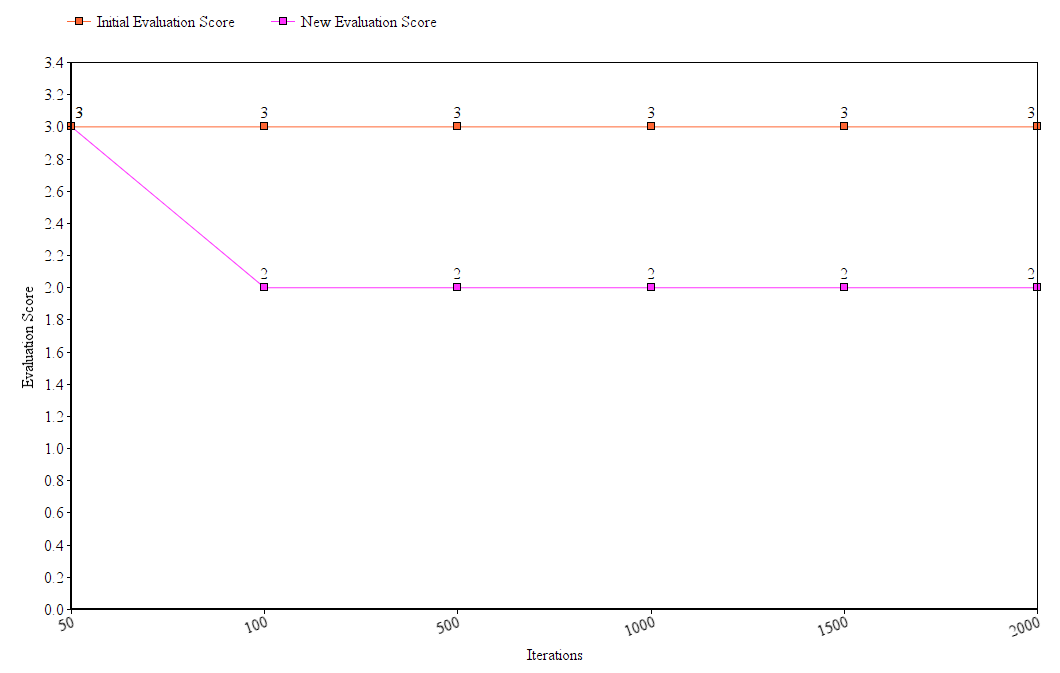
\includegraphics[width=100mm]{5x5Path.png}
\caption{5x5 Data with Path}
\label{fig:method}
\end{figure}

\begin{figure}[H]
\centering
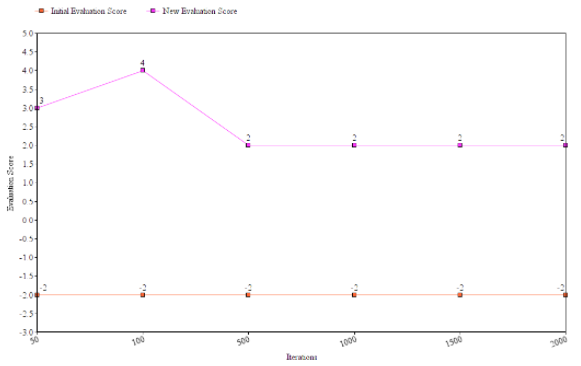
\includegraphics[width=100mm]{5x5noPath.png}
\caption{5x5 Data without Path}
\label{fig:method}
\end{figure}
%7x7 Grid
\begin{figure}[H]
\centering
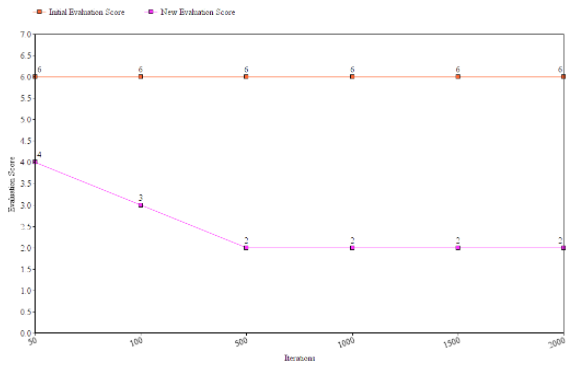
\includegraphics[width=100mm]{7x7Path.png}
\caption{7x7 Data with Path}
\label{fig:method}
\end{figure}

\begin{figure}[H]
\centering
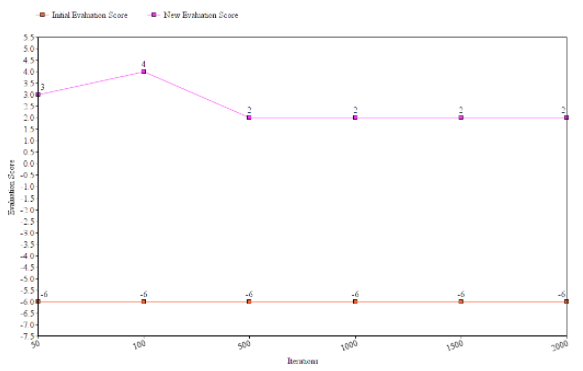
\includegraphics[width=100mm]{7x7noPath.png}
\caption{7x7 Data without Path}
\label{fig:method}
\end{figure}

%9x9 Grid
\begin{figure}[H]
\centering
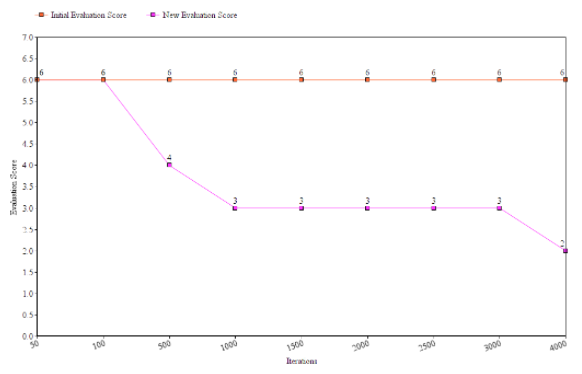
\includegraphics[width=100mm]{9x9Path.png}
\caption{9x9 Data with Path}
\label{fig:method}
\end{figure}

\begin{figure}[H]
\centering
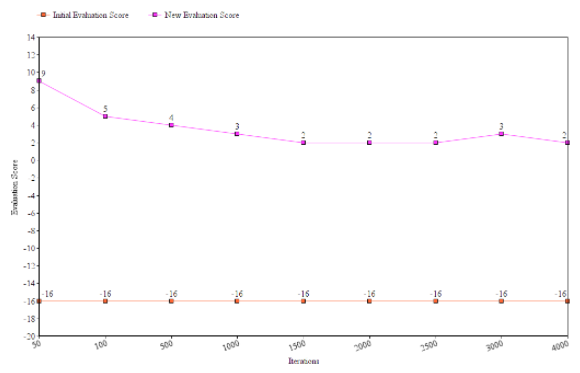
\includegraphics[width=100mm]{9x9noPath.png}
\caption{9x9 Data without Path}
\label{fig:method}
\end{figure}

%11x11 Grid 
\begin{figure}[H]
\centering
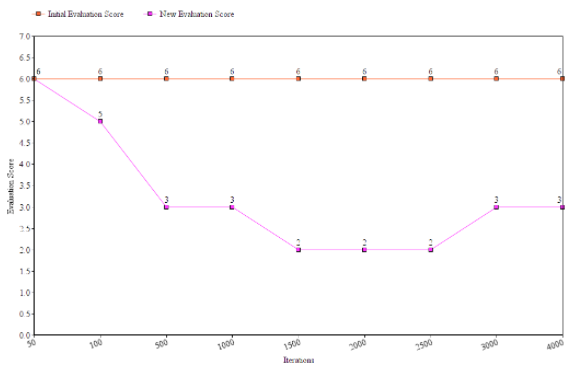
\includegraphics[width=100mm]{11x11Path.png}
\caption{11x11 Data with Path}
\label{fig:method}
\end{figure}

\begin{figure}[H]
\centering
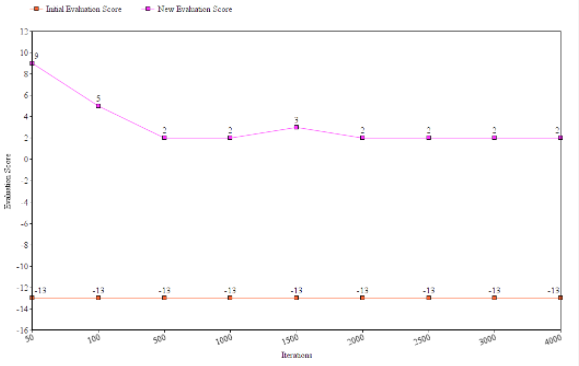
\includegraphics[width=100mm]{11x11noPath.png}
\caption{11x11 Data without Path}
\label{fig:method}
\end{figure}

It was concluded from the data for each of the different sized grids that as the grid dimensions grew, it took more iterations for the Hill Climb to result in an optimal state where the evaluation score was 2 (the best possible score). Also, it was found that the grids that did not have a path initially resulted in an evaluation score of 2 faster than those that already had paths.

\section{Task 4 - 6}

Tasks 4-6 are run using the Task 4 - 6 textfields and solve button. The user must input: Number of Restarts, Hill Climb Iterations, Probability of a Downstep, Initial Temperature, and Temperature Decay Rate. Once the user does this and clicks the solve button, all four grids for Pure Hill Climb, Hill Climb with Random Restarts, Hill Climb with Random Walk, and Simulated Annealing are displayed in the GUI. Underneath each grid is the corresponding data for that grid: initial evaluation function, resulting evaluation function, and time elapsed.

\subsection{Task 4}
The Task 4 is completed by taking the data from the random restarts and the iterations text fields that the user has input. The grid that represents the hill climbs performs the hill climbing process for the specified number of iterations. We divide the number of iterations by the number of restarts to give us the number of iterations to perform the hill climbing process before restarting from a new puzzle state.

We have plotted data for each of the different sized grids.

%5x5 Grid with Path
\begin{figure}[H]
\centering
\begin{subfigure}{.5\textwidth}
	\centering
	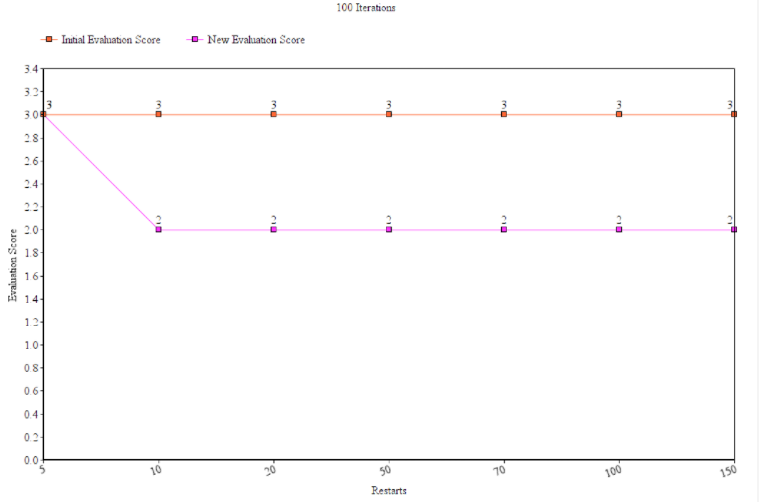
\includegraphics[width=50mm]{5x5restart.png}
	\caption{5x5 Data with 100 iterations and Initial Path}
	\label{fig:method}
\end{subfigure}%
\begin{subfigure}{.5\textwidth}
	\centering
	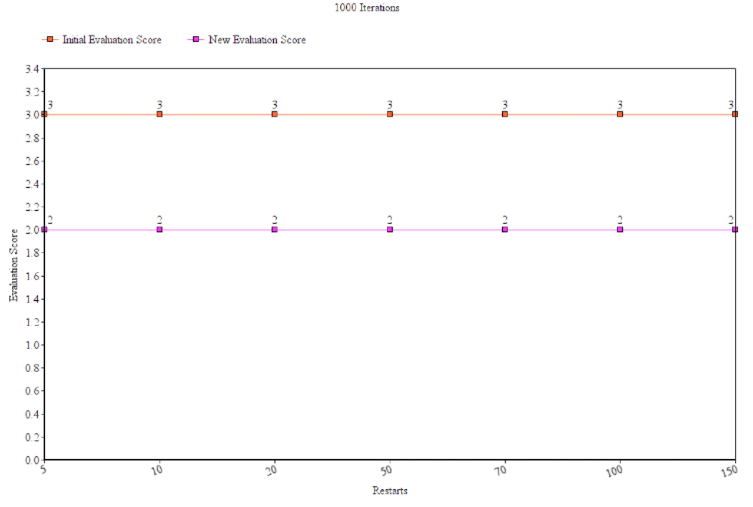
\includegraphics[width=50mm]{5x5restart2.png}
	\caption{5x5 Data with 1000 iterations and Initial Path}
	\label{fig:method}
\end{subfigure}
\end{figure}

%5x5 Grid without Path
\begin{figure}[H]
\centering
\begin{subfigure}{.5\textwidth}
	\centering
	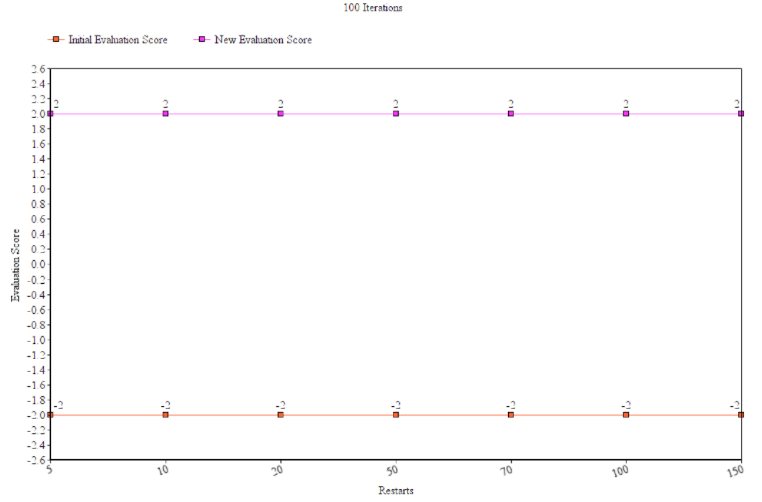
\includegraphics[width=50mm]{5x5restPath.png}
	\caption{5x5 Data with 100 iterations and No Initial Path}
	\label{fig:method}
\end{subfigure}%
\begin{subfigure}{.5\textwidth}
	\centering
	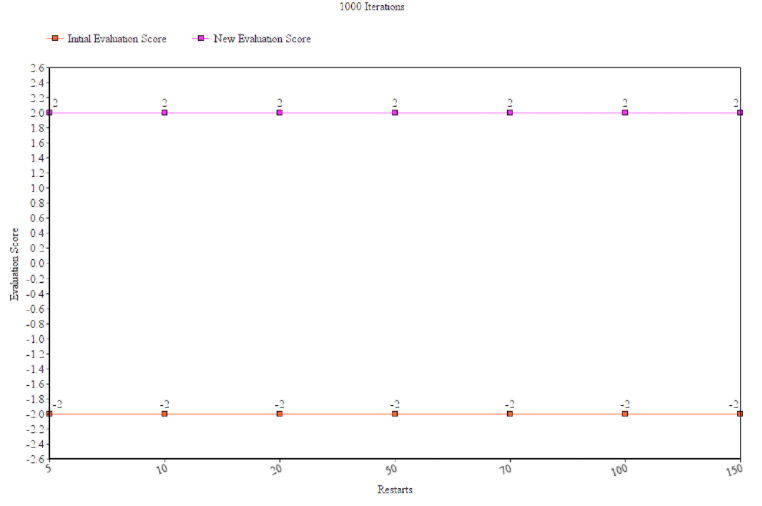
\includegraphics[width=50mm]{5x5restPath2.png}
	\caption{5x5 Data with 1000 iterations and No Initial Path}
	\label{fig:method}
\end{subfigure}
\end{figure}

%7x7 Grid with Path
\begin{figure}[H]
\centering
\begin{subfigure}{.5\textwidth}
	\centering
	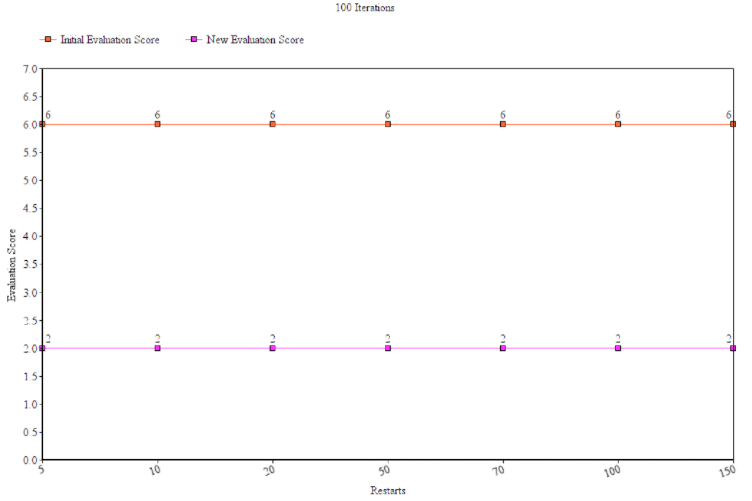
\includegraphics[width=50mm]{7x7restart.png}
	\caption{7x7 Data with 100 iterations and Initial Path}
	\label{fig:method}
\end{subfigure}%
\begin{subfigure}{.5\textwidth}
	\centering
	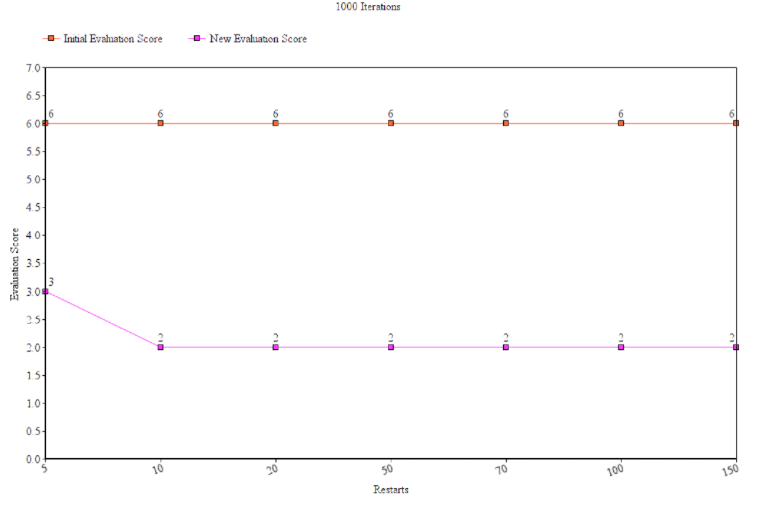
\includegraphics[width=50mm]{7x7restart2.png}
	\caption{7x7 Data with 1000 iterations and Initial Path}
	\label{fig:method}
\end{subfigure}
\end{figure}

%7x7 Grid without Path
\begin{figure}[H]
\centering
\begin{subfigure}{.5\textwidth}
	\centering
	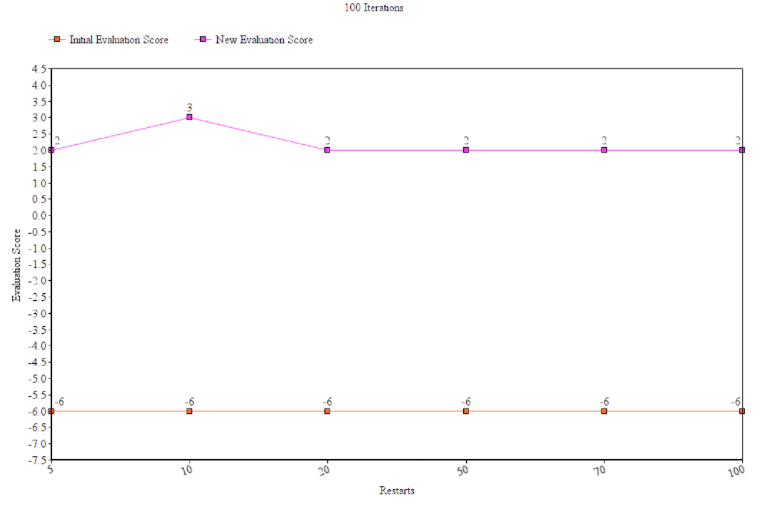
\includegraphics[width=50mm]{7x7restPath.png}
	\caption{7x7 Data with 100 iterations and No Initial Path}
	\label{fig:method}
\end{subfigure}%
\begin{subfigure}{.5\textwidth}
	\centering
	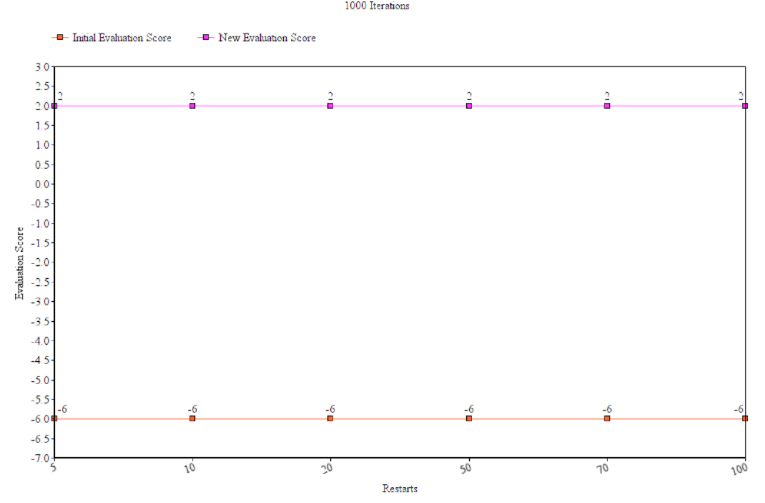
\includegraphics[width=50mm]{7x7restPath2.png}
	\caption{7x7 Data with 1000 iterations and No Initial Path}
	\label{fig:method}
\end{subfigure}
\end{figure}

%9x9 Grid with Path
\begin{figure}[H]
\centering
\begin{subfigure}{.5\textwidth}
	\centering
	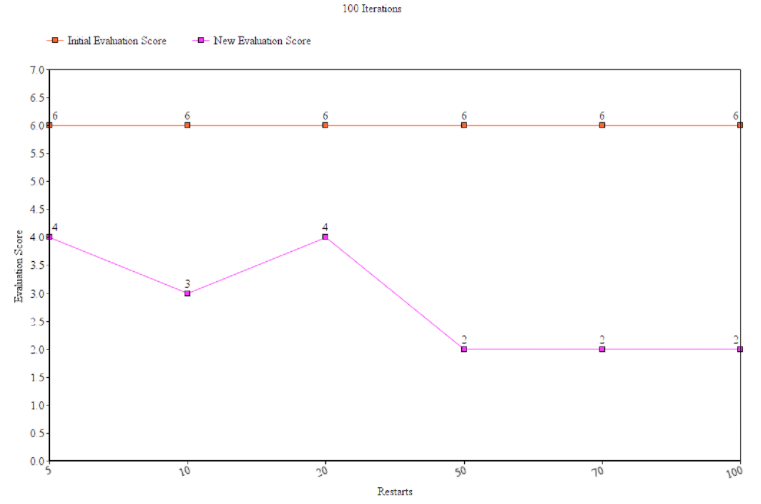
\includegraphics[width=50mm]{9x9restart.png}
	\caption{9x9 Data with 100 iterations and Initial Path}
	\label{fig:method}
\end{subfigure}%
\begin{subfigure}{.5\textwidth}
	\centering
	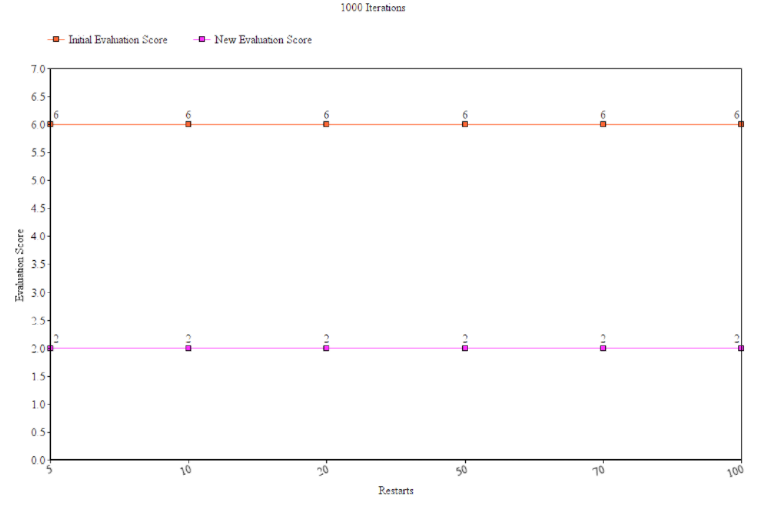
\includegraphics[width=50mm]{9x9restart2.png}
	\caption{9x9 Data with 1000 iterations and Initial Path}
	\label{fig:method}
\end{subfigure}
\end{figure}

%9x9 Grid without Path
\begin{figure}[H]
\centering
\begin{subfigure}{.5\textwidth}
	\centering
	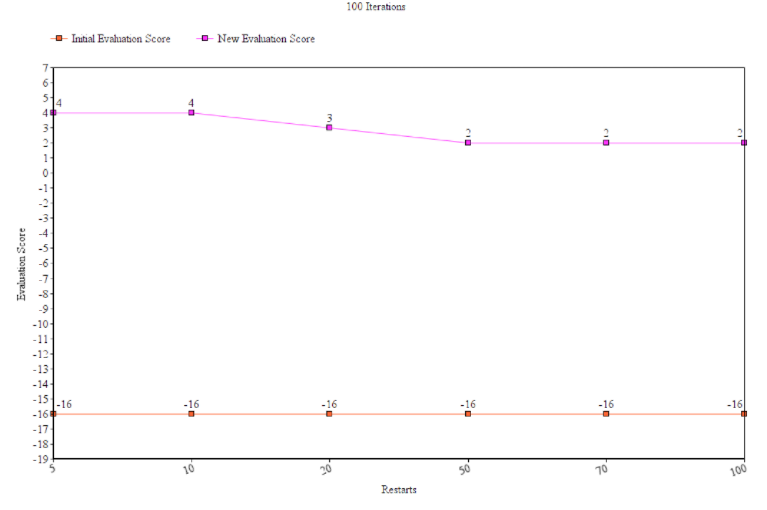
\includegraphics[width=50mm]{9x9restPath.png}
	\caption{9x9 Data with 100 iterations and No Initial Path}
	\label{fig:method}
\end{subfigure}%
\begin{subfigure}{.5\textwidth}
	\centering
	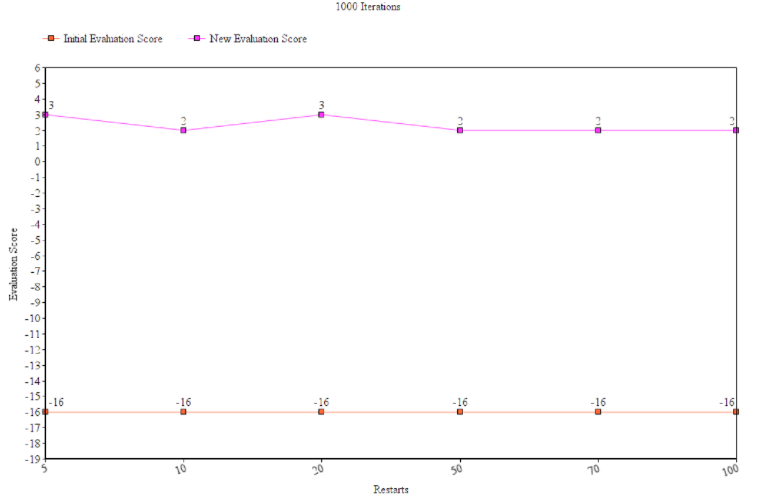
\includegraphics[width=50mm]{9x9restPath2.png}
	\caption{9x9 Data with 1000 iterations and No Initial Path}
	\label{fig:method}
\end{subfigure}
\end{figure}

%11x11 Grid with Path
\begin{figure}[H]
\centering
\begin{subfigure}{.5\textwidth}
	\centering
	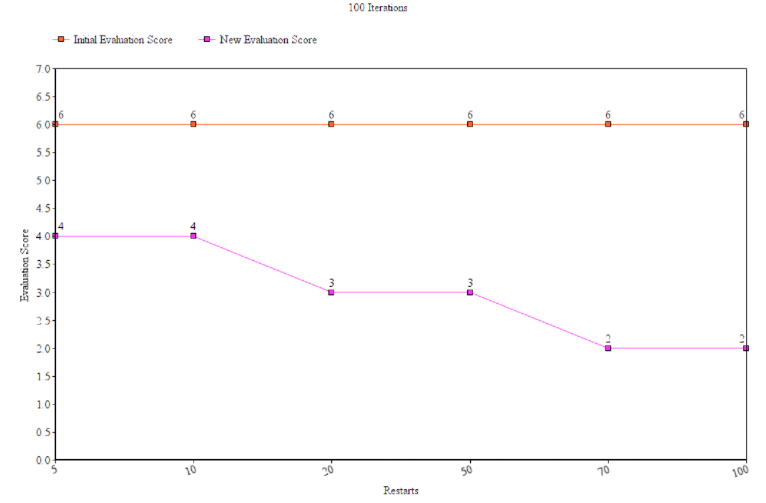
\includegraphics[width=50mm]{11x11restart.png}
	\caption{11x11 Data with 100 iterations and Initial Path}
	\label{fig:method}
\end{subfigure}%
\begin{subfigure}{.5\textwidth}
	\centering
	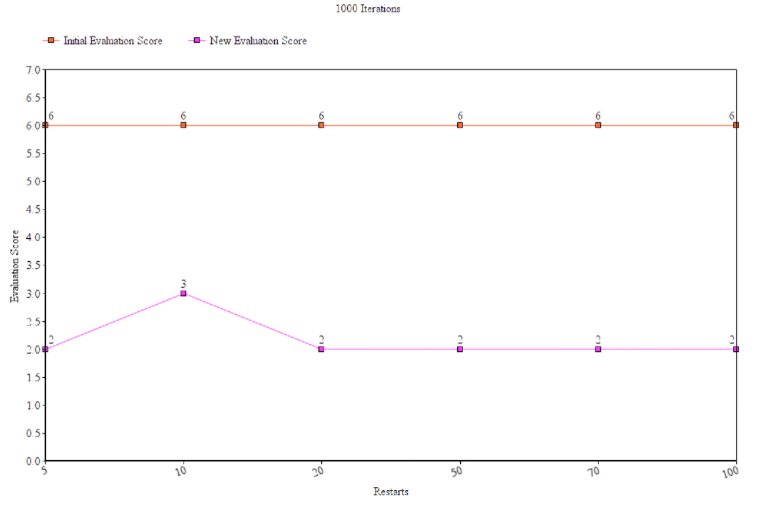
\includegraphics[width=50mm]{11x11restart2.png}
	\caption{11x11 Data with 1000 iterations and Initial Path}
	\label{fig:method}
\end{subfigure}
\end{figure}

%11x11 Grid without Path
\begin{figure}[H]
\centering
\begin{subfigure}{.5\textwidth}
	\centering
	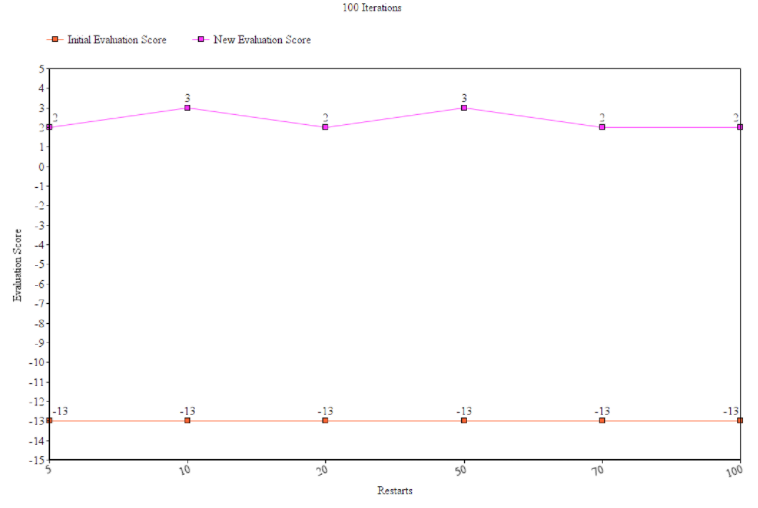
\includegraphics[width=50mm]{11x11restPath.png}
	\caption{11x11 Data with 100 iterations and No Initial Path}
	\label{fig:method}
\end{subfigure}%
\begin{subfigure}{.5\textwidth}
	\centering
	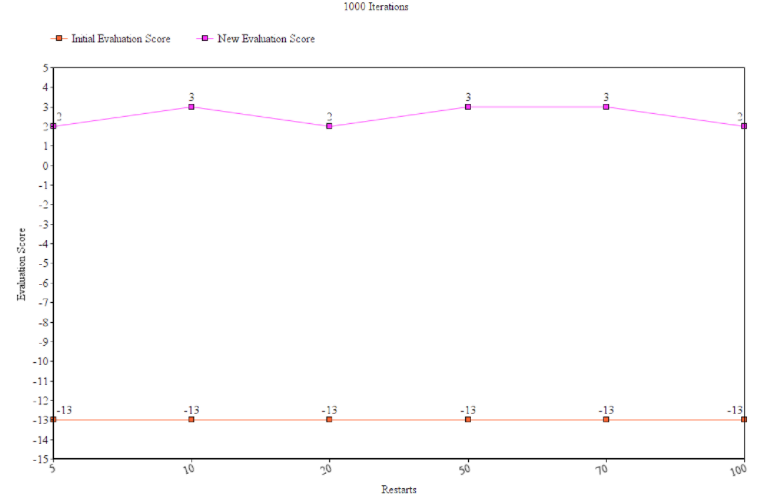
\includegraphics[width=50mm]{11x11restPath2.png}
	\caption{11x11 Data with 1000 iterations and No Initial Path}
	\label{fig:method}
\end{subfigure}
\end{figure}

We conclude that Local Search reaches the optimal amount of steps to the goal, 2, faster with a large number of iterations than with a small number of iterations. The Pure Hill Climb is better to use when the iterations are high, but the Hill Climb with Random Restarts is better when the iterations are low.

\subsection{Task 5}
Task 5 is completed by taking the data from the iterations and probability of a downstep text fields that the user has input. It asks the user to input the number of iterations for hill climb, and the probability $p$ that the program will accept a worse state during an iteration.

We have plotted data for each of the different sized grids.

%5x5 Grid with Path
\begin{figure}[H]
\centering
\begin{subfigure}{.5\textwidth}
	\centering
	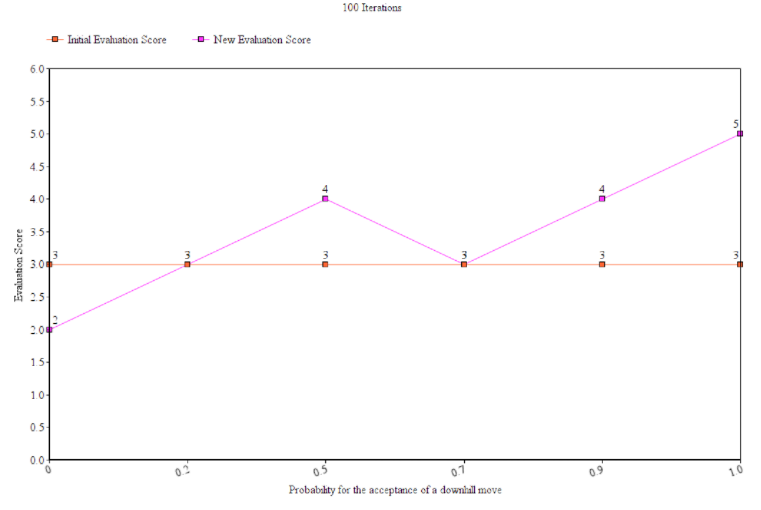
\includegraphics[width=50mm]{5x5down.png}
	\caption{5x5 Data with 100 iterations and Initial Path}
	\label{fig:method}
\end{subfigure}%
\begin{subfigure}{.5\textwidth}
	\centering
	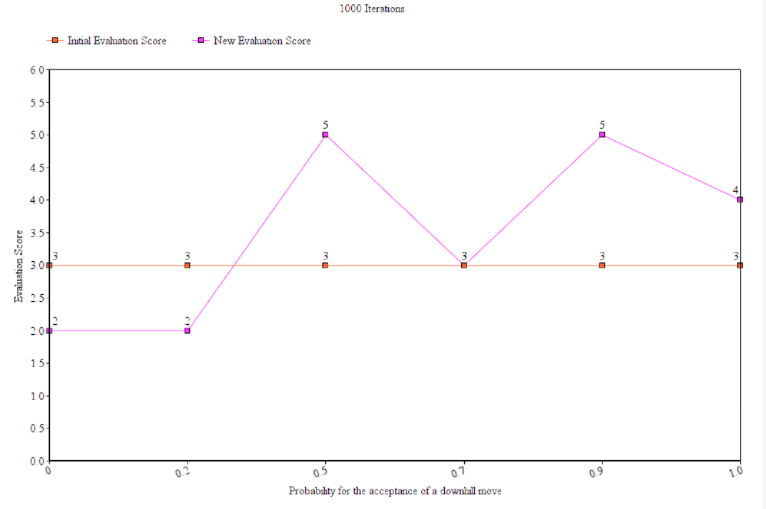
\includegraphics[width=50mm]{5x5down2.png}
	\caption{5x5 Data with 1000 iterations and Initial Path}
	\label{fig:method}
\end{subfigure}
\end{figure}

%5x5 Grid without Path
\begin{figure}[H]
\centering
\begin{subfigure}{.5\textwidth}
	\centering
	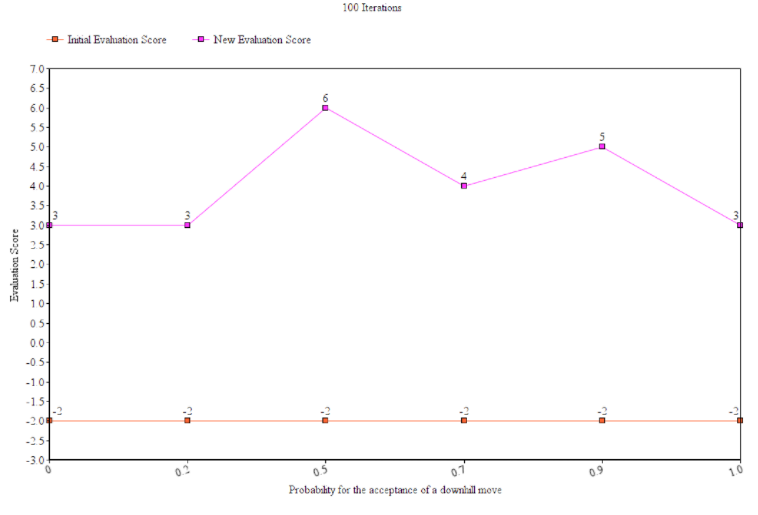
\includegraphics[width=50mm]{5x5downPath.png}
	\caption{5x5 Data with 100 iterations and No Initial Path}
	\label{fig:method}
\end{subfigure}%
\begin{subfigure}{.5\textwidth}
	\centering
	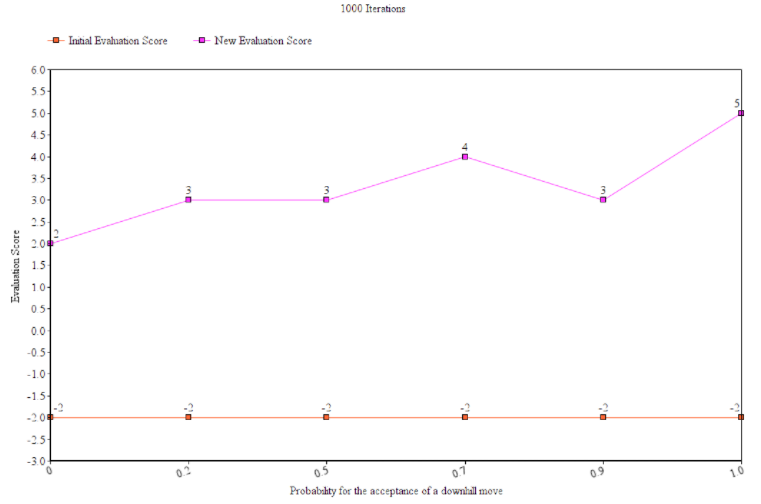
\includegraphics[width=50mm]{5x5downPath2.png}
	\caption{5x5 Data with 1000 iterations and No Initial Path}
	\label{fig:method}
\end{subfigure}
\end{figure}

%7x7 Grid with Path
\begin{figure}[H]
\centering
\begin{subfigure}{.5\textwidth}
	\centering
	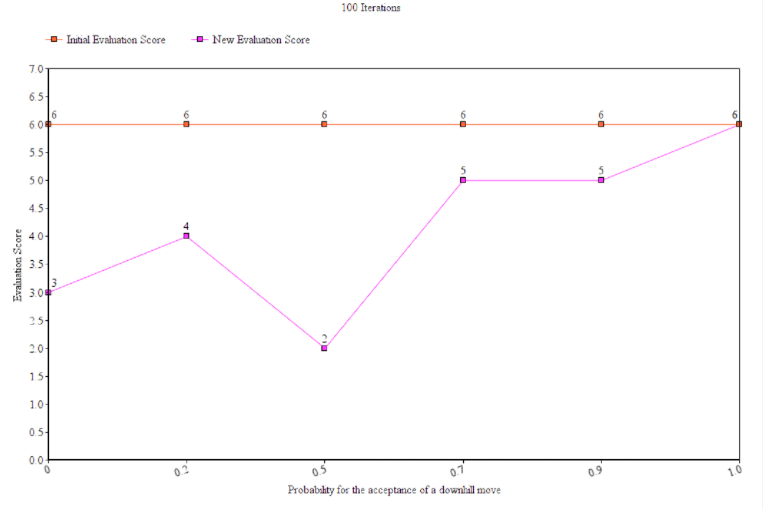
\includegraphics[width=50mm]{7x7down.png}
	\caption{7x7 Data with 100 iterations and Initial Path}
	\label{fig:method}
\end{subfigure}%
\begin{subfigure}{.5\textwidth}
	\centering
	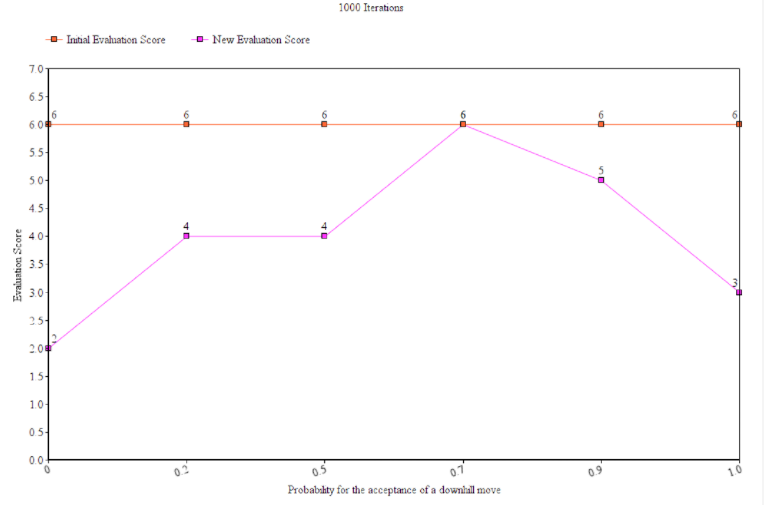
\includegraphics[width=50mm]{7x7down2.png}
	\caption{7x7 Data with 1000 iterations and Initial Path}
	\label{fig:method}
\end{subfigure}
\end{figure}

%7x7 Grid without Path
\begin{figure}[H]
\centering
\begin{subfigure}{.5\textwidth}
	\centering
	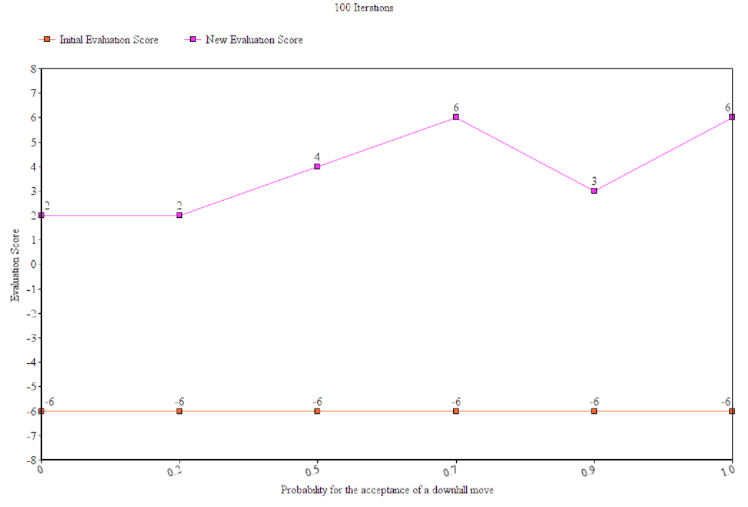
\includegraphics[width=50mm]{7x7downPath.png}
	\caption{7x7 Data with 100 iterations and No Initial Path}
	\label{fig:method}
\end{subfigure}%
\begin{subfigure}{.5\textwidth}
	\centering
	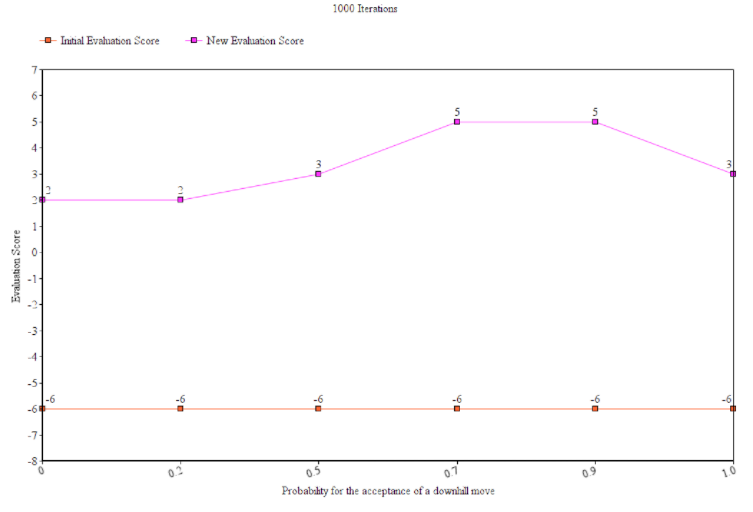
\includegraphics[width=50mm]{7x7downPath2.png}
	\caption{7x7 Data with 1000 iterations and No Initial Path}
	\label{fig:method}
\end{subfigure}
\end{figure}

%9x9 Grid with Path
\begin{figure}[H]
\centering
\begin{subfigure}{.5\textwidth}
	\centering
	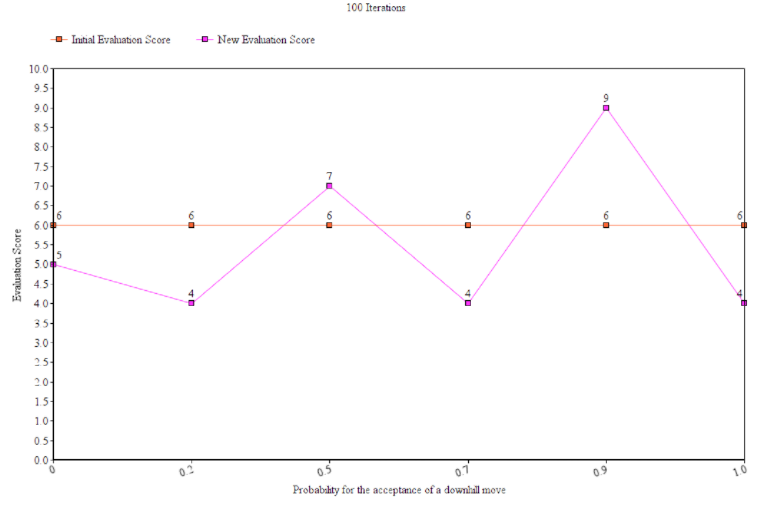
\includegraphics[width=50mm]{9x9down.png}
	\caption{9x9 Data with 100 iterations and Initial Path}
	\label{fig:method}
\end{subfigure}%
\begin{subfigure}{.5\textwidth}
	\centering
	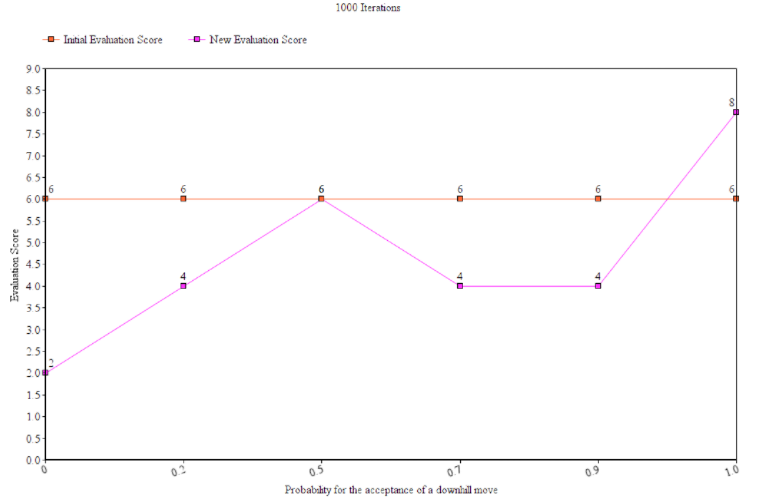
\includegraphics[width=50mm]{9x9down2.png}
	\caption{9x9 Data with 1000 iterations and Initial Path}
	\label{fig:method}
\end{subfigure}
\end{figure}

%9x9 Grid without Path
\begin{figure}[H]
\centering
\begin{subfigure}{.5\textwidth}
	\centering
	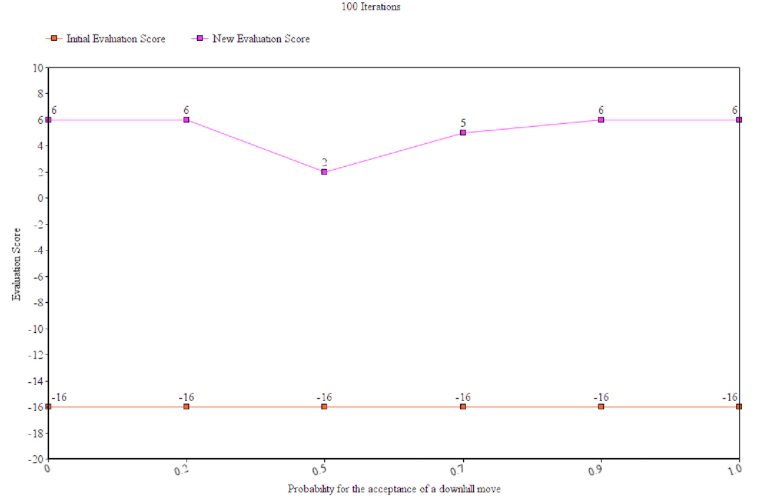
\includegraphics[width=50mm]{9x9downPath.png}
	\caption{9x9 Data with 100 iterations and No Initial Path}
	\label{fig:method}
\end{subfigure}%
\begin{subfigure}{.5\textwidth}
	\centering
	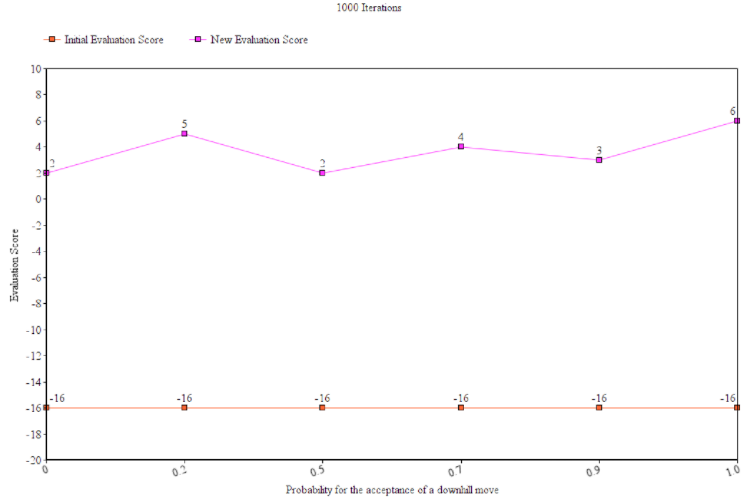
\includegraphics[width=50mm]{9x9downPath2.png}
	\caption{9x9 Data with 1000 iterations and No Initial Path}
	\label{fig:method}
\end{subfigure}
\end{figure}

%11x11 Grid with Path
\begin{figure}[H]
\centering
\begin{subfigure}{.5\textwidth}
	\centering
	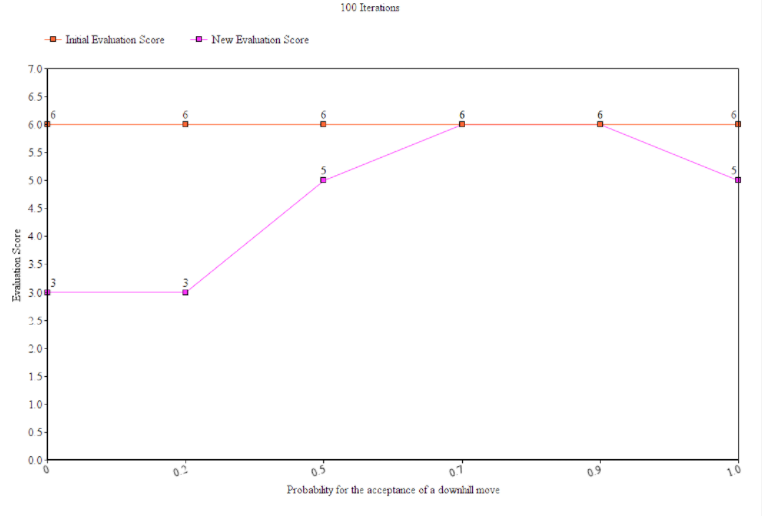
\includegraphics[width=50mm]{11x11down.png}
	\caption{11x11 Data with 100 iterations and Initial Path}
	\label{fig:method}
\end{subfigure}%
\begin{subfigure}{.5\textwidth}
	\centering
	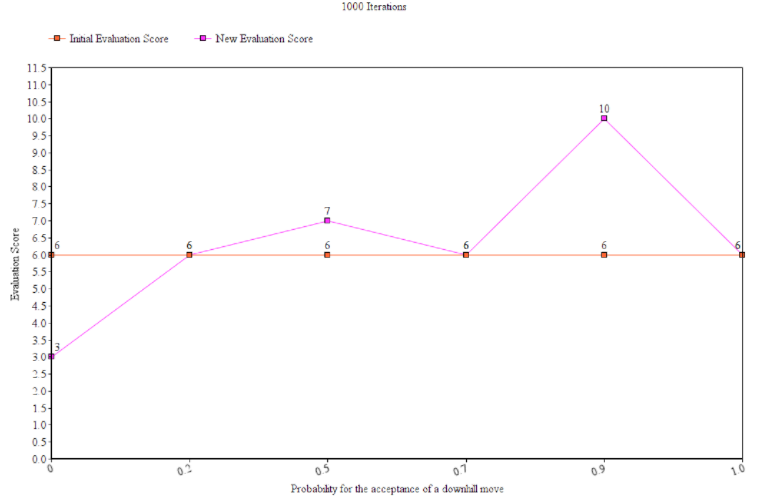
\includegraphics[width=50mm]{11x11down2.png}
	\caption{11x11 Data with 1000 iterations and Initial Path}
	\label{fig:method}
\end{subfigure}
\end{figure}

%11x11 Grid without Path
\begin{figure}[H]
\centering
\begin{subfigure}{.5\textwidth}
	\centering
	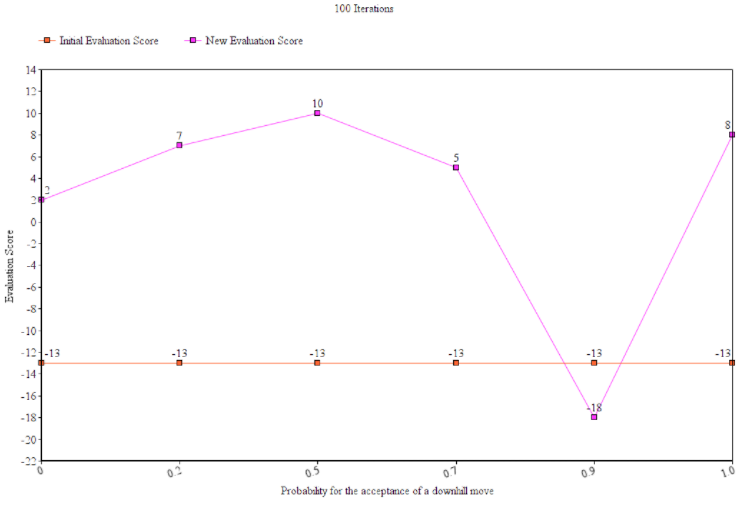
\includegraphics[width=50mm]{11x11downPath.png}
	\caption{11x11 Data with 100 iterations and No Initial Path}
	\label{fig:method}
\end{subfigure}%
\begin{subfigure}{.5\textwidth}
	\centering
	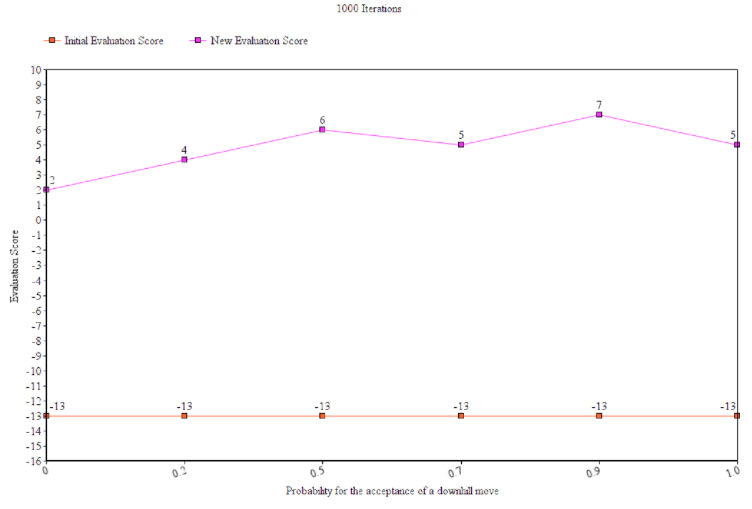
\includegraphics[width=50mm]{11x11downPath2.png}
	\caption{11x11 Data with 1000 iterations and No Initial Path}
	\label{fig:method}
\end{subfigure}
\end{figure}

We conclude that with a lower probability you are more likely to optimize the puzzle and lower your evaluation score. As the probability increases, you are more likely to make your puzzle worse than it initially was. Also, with a larger number of iterations and larger probability to step down, the evaluation score tends to become much worse by increasing the evaluation score. One graph even shows that a puzzle became unsolvable with no path.

\subsection{Task 6}
Task 6 is completed by taking the data from the iterations, initial temperature, and the temperature decay rate text fields that the user inputs. In the beginning, simulated annealing is more likely to accept a lower state but as the temperature decays it becomes more strict with pure hill climbing.

We have plotted data for each of the different sized grids.

%5x5 Grid with Path
%Low Iterations and Low Temperature
\begin{figure}[H]
\centering
\begin{subfigure}{.5\textwidth}
	\centering
	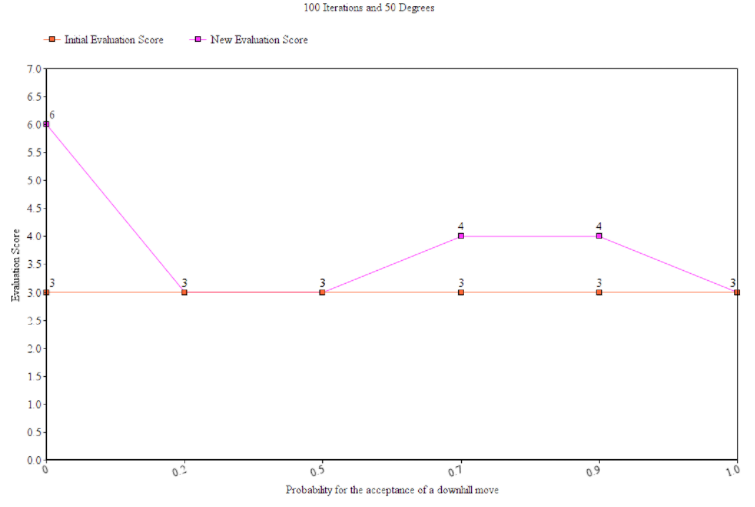
\includegraphics[width=50mm]{5x5lowIlowT.png}
	\caption{5x5 Data with Initial Path}
	\label{fig:method}
\end{subfigure}%
\begin{subfigure}{.5\textwidth}
	\centering
	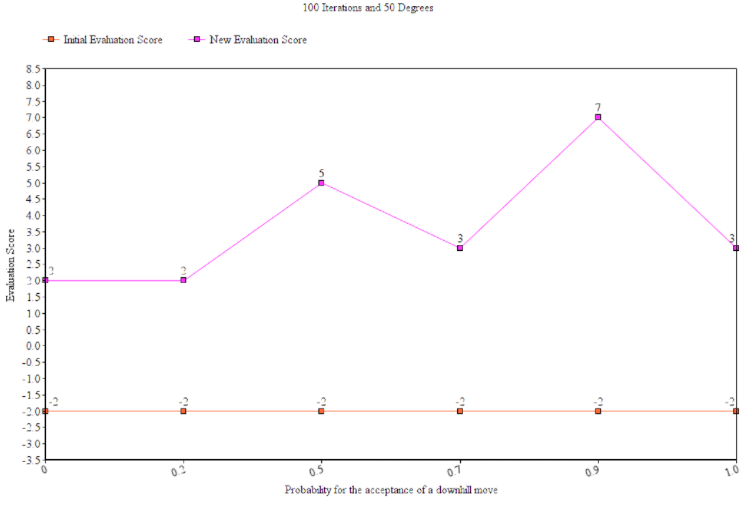
\includegraphics[width=50mm]{5x5lowIlowTPath.png}
	\caption{5x5 Data with No Initial Path}
	\label{fig:method}
\end{subfigure}
\caption{100 Iterations and 50 Degrees}
\end{figure}

%5x5 Grid with Path
%High Iterations and Low Temperature
\begin{figure}[H]
\centering
\begin{subfigure}{.5\textwidth}
	\centering
	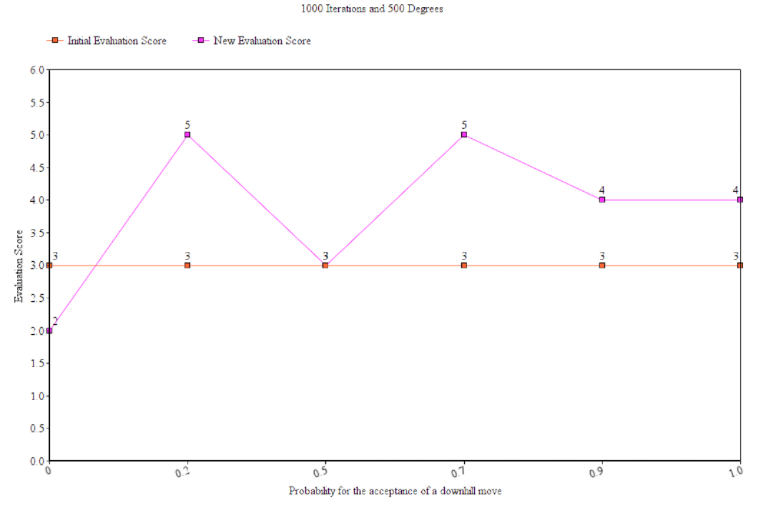
\includegraphics[width=50mm]{5x5highIhighT.png}
	\caption{5x5 Data with Initial Path}
	\label{fig:method}
\end{subfigure}%
\begin{subfigure}{.5\textwidth}
	\centering
	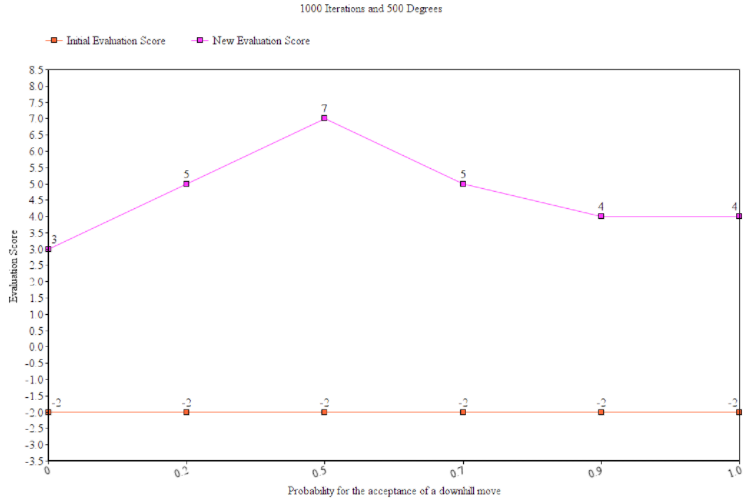
\includegraphics[width=50mm]{5x5highIhighTPath.png}
	\caption{5x5 Data with No Initial Path}
	\label{fig:method}
\end{subfigure}
\caption{1000 Iterations and 50 Degrees}
\end{figure}

%5x5 Grid with Path
%Low Iterations and High Temperature
\begin{figure}[H]
\centering
\begin{subfigure}{.5\textwidth}
	\centering
	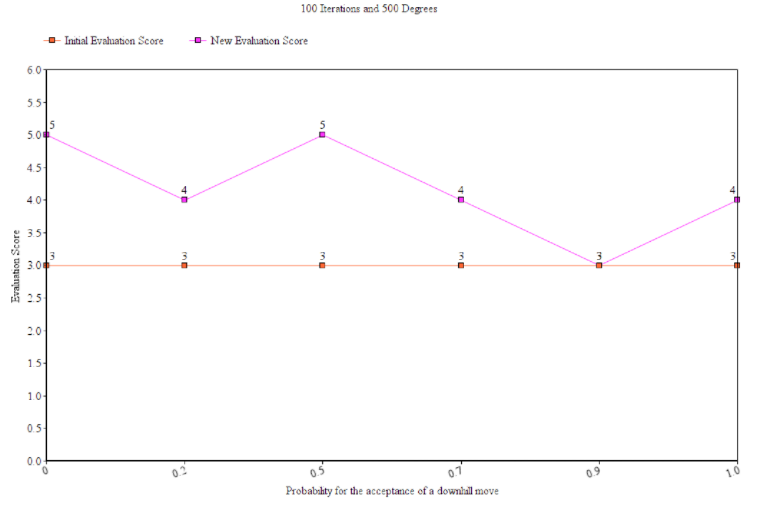
\includegraphics[width=50mm]{5x5lowIhighT.png}
	\caption{5x5 Data with Initial Path}
	\label{fig:method}
\end{subfigure}%
\begin{subfigure}{.5\textwidth}
	\centering
	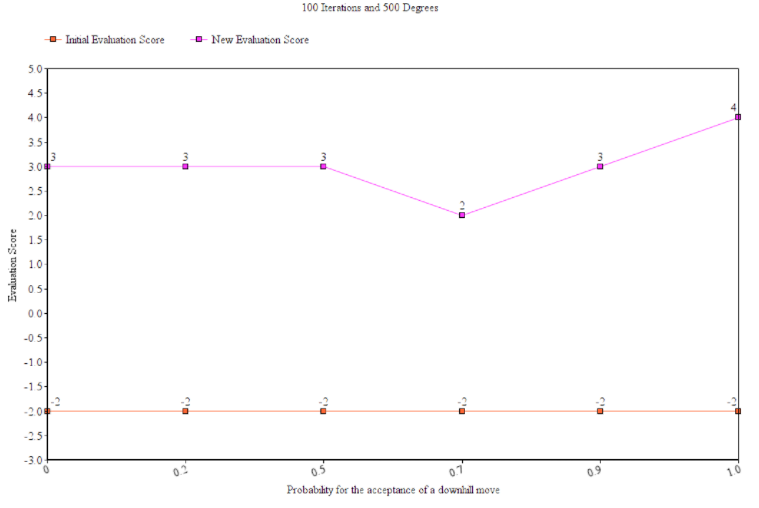
\includegraphics[width=50mm]{5x5lowIhighTPath.png}
	\caption{5x5 Data with No Initial Path}
	\label{fig:method}
\end{subfigure}
\caption{100 Iterations and 500 Degrees}
\end{figure}

%5x5 Grid with Path
%High Iterations and High Temperature
\begin{figure}[H]
\centering
\begin{subfigure}{.5\textwidth}
	\centering
	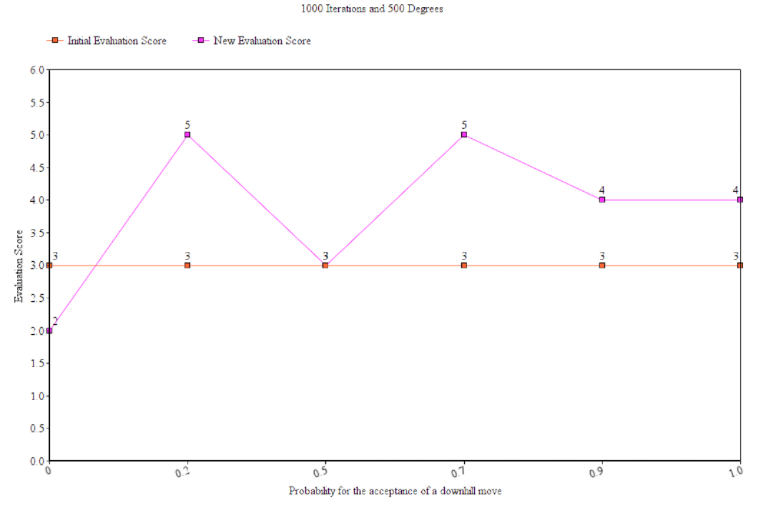
\includegraphics[width=50mm]{5x5highIhighT.png}
	\caption{5x5 Data with Initial Path}
	\label{fig:method}
\end{subfigure}%
\begin{subfigure}{.5\textwidth}
	\centering
	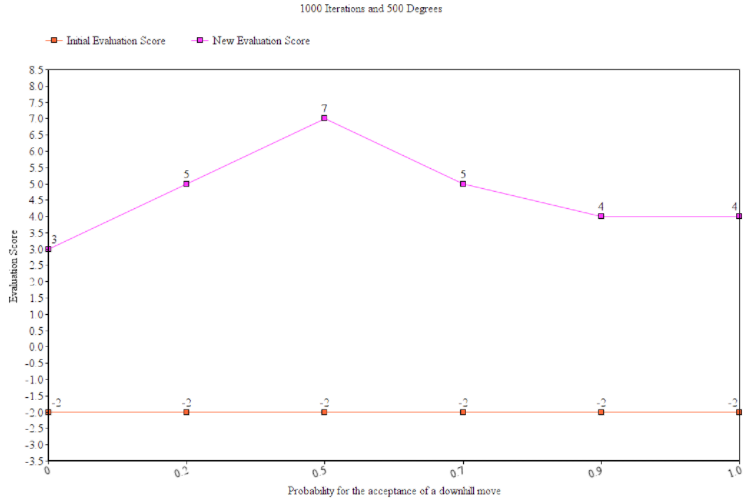
\includegraphics[width=50mm]{5x5highIhighTPath.png}
	\caption{5x5 Data with No Initial Path}
	\label{fig:method}
\end{subfigure}
\caption{1000 Iterations and 500 Degrees}
\end{figure}

%7x7 Grid with Path
%Low Iterations and Low Temperature
\begin{figure}[H]
\centering
\begin{subfigure}{.5\textwidth}
	\centering
	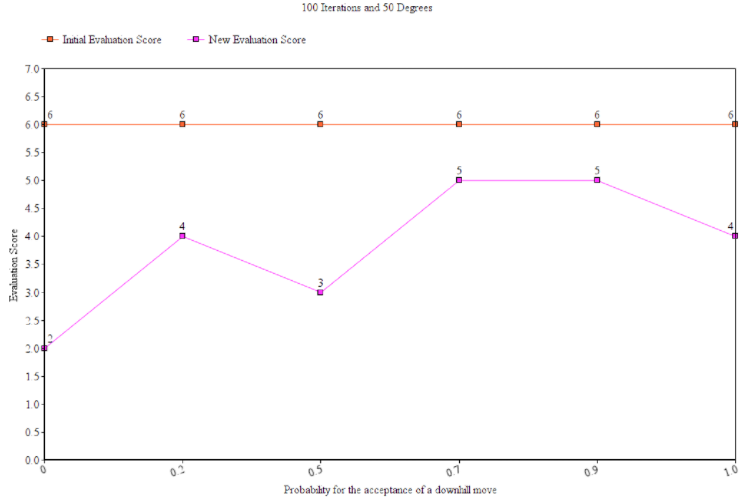
\includegraphics[width=50mm]{7x7lowIlowT.png}
	\caption{7x7 Data with Initial Path}
	\label{fig:method}
\end{subfigure}%
\begin{subfigure}{.5\textwidth}
	\centering
	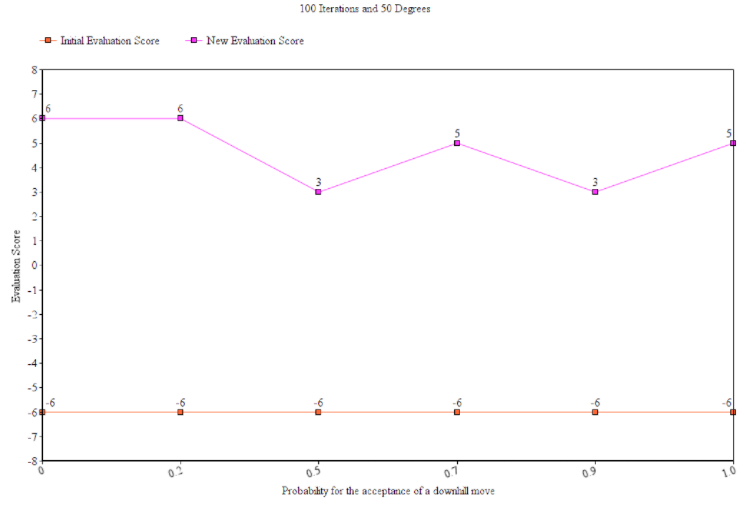
\includegraphics[width=50mm]{7x7lowIlowTPath.png}
	\caption{7x7 Data with No Initial Path}
	\label{fig:method}
\end{subfigure}
\caption{100 Iterations and 50 Degrees}
\end{figure}

%7x7 Grid with Path
%High Iterations and Low Temperature
\begin{figure}[H]
\centering
\begin{subfigure}{.5\textwidth}
	\centering
	\includegraphics[width=50mm]{7x7highIhighT.png}
	\caption{7x7 Data with Initial Path}
	\label{fig:method}
\end{subfigure}%
\begin{subfigure}{.5\textwidth}
	\centering
	\includegraphics[width=50mm]{7x7highIhighTPath.png}
	\caption{7x7 Data with No Initial Path}
	\label{fig:method}
\end{subfigure}
\caption{1000 Iterations and 50 Degrees}
\end{figure}

%7x7 Grid with Path
%Low Iterations and High Temperature
\begin{figure}[H]
\centering
\begin{subfigure}{.5\textwidth}
	\centering
	\includegraphics[width=50mm]{7x7lowIhighT.png}
	\caption{7x7 Data with Initial Path}
	\label{fig:method}
\end{subfigure}%
\begin{subfigure}{.5\textwidth}
	\centering
	\includegraphics[width=50mm]{7x7lowIhighTPath.png}
	\caption{7x7 Data with No Initial Path}
	\label{fig:method}
\end{subfigure}
\caption{100 Iterations and 500 Degrees}
\end{figure}

%7x7 Grid with Path
%High Iterations and High Temperature
\begin{figure}[H]
\centering
\begin{subfigure}{.5\textwidth}
	\centering
	\includegraphics[width=50mm]{7x7highIhighT.png}
	\caption{7x7 Data with Initial Path}
	\label{fig:method}
\end{subfigure}%
\begin{subfigure}{.5\textwidth}
	\centering
	\includegraphics[width=50mm]{7x7highIhighTPath.png}
	\caption{7x7 Data with No Initial Path}
	\label{fig:method}
\end{subfigure}
\caption{1000 Iterations and 500 Degrees}
\end{figure}

%9x9 Grid with Path
%Low Iterations and Low Temperature
\begin{figure}[H]
\centering
\begin{subfigure}{.5\textwidth}
	\centering
	\includegraphics[width=50mm]{9x9lowIlowT.png}
	\caption{9x9 Data with Initial Path}
	\label{fig:method}
\end{subfigure}%
\begin{subfigure}{.5\textwidth}
	\centering
	\includegraphics[width=50mm]{9x9lowIlowTPath.png}
	\caption{9x9 Data with No Initial Path}
	\label{fig:method}
\end{subfigure}
\caption{100 Iterations and 50 Degrees}
\end{figure}

%9x9 Grid with Path
%High Iterations and Low Temperature
\begin{figure}[H]
\centering
\begin{subfigure}{.5\textwidth}
	\centering
	\includegraphics[width=50mm]{9x9highIhighT.png}
	\caption{9x9 Data with Initial Path}
	\label{fig:method}
\end{subfigure}%
\begin{subfigure}{.5\textwidth}
	\centering
	\includegraphics[width=50mm]{9x9highIhighTPath.png}
	\caption{9x9 Data with No Initial Path}
	\label{fig:method}
\end{subfigure}
\caption{1000 Iterations and 50 Degrees}
\end{figure}

%9x9 Grid with Path
%Low Iterations and High Temperature
\begin{figure}[H]
\centering
\begin{subfigure}{.5\textwidth}
	\centering
	\includegraphics[width=50mm]{9x9lowIhighT.png}
	\caption{9x9 Data with Initial Path}
	\label{fig:method}
\end{subfigure}%
\begin{subfigure}{.5\textwidth}
	\centering
	\includegraphics[width=50mm]{9x9lowIhighTPath.png}
	\caption{9x9 Data with No Initial Path}
	\label{fig:method}
\end{subfigure}
\caption{100 Iterations and 500 Degrees}
\end{figure}

%9x9 Grid with Path
%High Iterations and High Temperature
\begin{figure}[H]
\centering
\begin{subfigure}{.5\textwidth}
	\centering
	\includegraphics[width=50mm]{9x9highIhighT.png}
	\caption{9x9 Data with Initial Path}
	\label{fig:method}
\end{subfigure}%
\begin{subfigure}{.5\textwidth}
	\centering
	\includegraphics[width=50mm]{9x9highIhighTPath.png}
	\caption{9x9 Data with No Initial Path}
	\label{fig:method}
\end{subfigure}
\caption{1000 Iterations and 500 Degrees}
\end{figure}

%11x11 Grid with Path
%Low Iterations and Low Temperature
\begin{figure}[H]
\centering
\begin{subfigure}{.5\textwidth}
	\centering
	\includegraphics[width=50mm]{11x11lowIlowT.png}
	\caption{11x11 Data with Initial Path}
	\label{fig:method}
\end{subfigure}%
\begin{subfigure}{.5\textwidth}
	\centering
	\includegraphics[width=50mm]{11x11lowIlowTPath.png}
	\caption{11x11 Data with No Initial Path}
	\label{fig:method}
\end{subfigure}
\caption{100 Iterations and 50 Degrees}
\end{figure}

%11x11 Grid with Path
%High Iterations and Low Temperature
\begin{figure}[H]
\centering
\begin{subfigure}{.5\textwidth}
	\centering
	\includegraphics[width=50mm]{11x11highIhighT.png}
	\caption{11x11 Data with Initial Path}
	\label{fig:method}
\end{subfigure}%
\begin{subfigure}{.5\textwidth}
	\centering
	\includegraphics[width=50mm]{11x11highIhighTPath.png}
	\caption{11x11 Data with No Initial Path}
	\label{fig:method}
\end{subfigure}
\caption{1000 Iterations and 50 Degrees}
\end{figure}

%11x11 Grid with Path
%Low Iterations and High Temperature
\begin{figure}[H]
\centering
\begin{subfigure}{.5\textwidth}
	\centering
	\includegraphics[width=50mm]{11x11lowIhighT.png}
	\caption{11x11 Data with Initial Path}
	\label{fig:method}
\end{subfigure}%
\begin{subfigure}{.5\textwidth}
	\centering
	\includegraphics[width=50mm]{11x11lowIhighTPath.png}
	\caption{11x11 Data with No Initial Path}
	\label{fig:method}
\end{subfigure}
\caption{100 Iterations and 500 Degrees}
\end{figure}

%11x11 Grid with Path
%High Iterations and High Temperature
\begin{figure}[H]
\centering
\begin{subfigure}{.5\textwidth}
	\centering
	\includegraphics[width=50mm]{11x11highIhighT.png}
	\caption{11x11 Data with Initial Path}
	\label{fig:method}
\end{subfigure}%
\begin{subfigure}{.5\textwidth}
	\centering
	\includegraphics[width=50mm]{11x11highIhighTPath.png}
	\caption{11x11 Data with No Initial Path}
	\label{fig:method}
\end{subfigure}
\caption{1000 Iterations and 500 Degrees}
\end{figure}

We concluded that with higher temperature and lower decay rate, Local Search optimizes faster but when the decay rate is higher we notice that the evaluation function becomes worse.

\section{Task 7}

For task 7, we used a genetic algorithm that accepts a randomly generated node with a probability proportional to its evaluation function. Two random puzzles were chosen with this probability to be deemed as parents for the upcoming generation. These parents would create two children in the crossover phase with a certain probability and these children would be added back into the population. Finally, the children would be mutated by a single grid cell value with a probability inputted by the user before being added back to the population. After a certain amount of generations, the most optimal puzzle configuration was chosen.

\end{document}  